\chapter[SCP-173 雕像]{
    SCP-173 The Sculpture - \bb{The Original}\\
    SCP-173 雕像 - \bb{最初之作}
}

\label{chap:SCP-173}

\heritage

\begin{figure}[H]
    \centering
    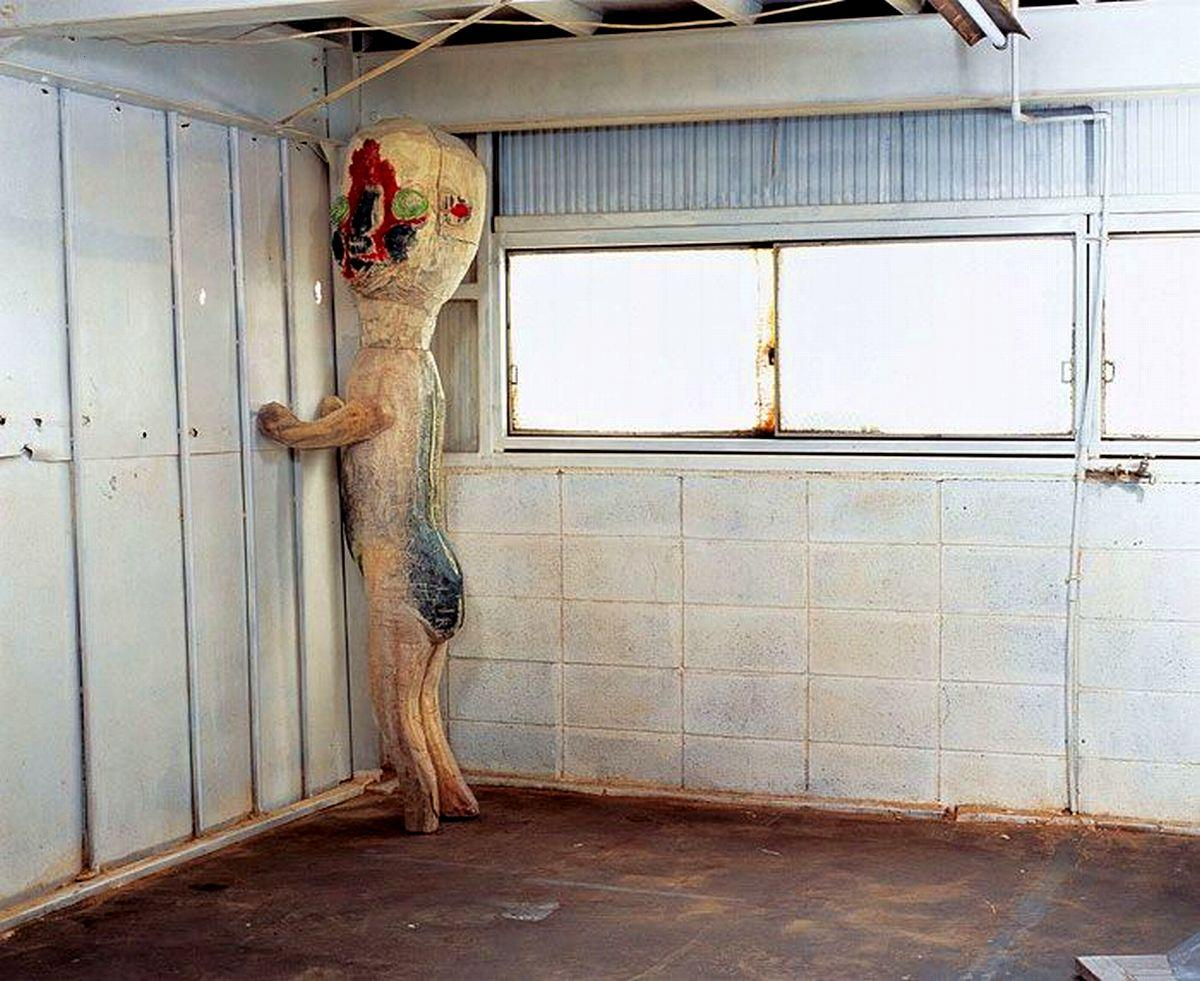
\includegraphics[width=0.5\linewidth]{images/SCP-173.jpg}
    \caption*{收容中的SCP-173}
\end{figure}

\bb{项目编号:}SCP-173

\bb{项目等级:}Euclid

\bb{特殊收容措施:}项目SCP-173应随时保存在一个上锁的收容区域内。如有人员必须进入SCP-173的收容区,人数须不少于三人,并且进入后必须锁上入口的门。至少两人必须随时与SCP-173保持眼神接触,直到所有人员离开、并将收容间重新上锁为止。

\bb{描述:}于1993年移动到Site-19,起源一直未知。它由混凝土和钢筋建造,并含有Krylon牌喷漆之痕迹。SCP-173是可动且带敌意的。项目在直接视线中不能移动。与SCP-173之间的视线绝不能在任何时候被中断,收容间内的人员必须在眨眼前相互给予指示。根据报告,项目以折断头骨与颈部相连之处或绞杀来攻击。在攻击事件中,人员需遵守第4级危险项目收容措施。

人员报告指出,在收容间无人时,其中会传出刮石声。此被认为是正常现象,并若有任何此种行为之改变,应当报告值班中的HMCL监督员处理。

在地板上的红棕色物质为粪便和血液组成,这些物质的来源未知。围墙须每两周清洁一次。

\hr

\bb{\uu{作者信息}}

\scriptsize{SCP-173中使用的图片是\href{http://izumikato.com/\#Untitled-2004}{Izumi Kato}创作的《Untitled 2004》系列艺术作品中的一张。该照片取自\href{http://www.scaithebathhouse.com/en/exhibitions/2005/04/izumi\_kato/}{Keisuke Yamamoto}。原作者保留所有权利。}

\scriptsize{提醒: SCP-173是对艺术作品 《Untitled 2004》的二次使用,由\href{http://izumikato.com/\#Untitled-2004}{Izumi Kato}创作。SCP-173的内容与艺术家作品《Untitled 2004》之内容没有任何关系。}

\scriptsize{该雕塑、其外形、其照片不适用于任何创作共用许可(Creative Commons license)。仅有该文章的文字部分适用创作共用。\bb{不得将该雕塑及其外形用作任何商业目的。Izumi Kato本人已慷慨地允许SCP Foundation及其爱好者团体以非商业目的使用《Untitled 2004》中的该图片。}}
